\chapter{Fast One-Ring Smoothing: Mathematical Grounding}
\label{ch4}
In this one, and the next two chapters, we present an updated version of \Fors{t}, based on the ideas initially proposed by H. Mara and S. Krömker at the EUROGRAPHICS Workshop on Graphics and Cultural Heritage (2017) ~\cite[s.~3.2]{Mara17}. Since publication, further research has been conducted by the authors, and it was determined that improvments to the weighting methods were possible, therefore, modifications to the algorithm were implemented directly within the GigaMesh \todoCitation{GigaMesh} framework. This chapter presents the mathematical grounding for the as-yet-unpublished version of \fors{t}, as it exists now in GigaMesh, with more accurate weighting methods based on the interpolation and extrapolation of function values to the center of gravity of each circular sector comprising the geodesic disc centered upon each point in a triangle mesh of \tdd{}.

The procedure for designing any convolutional filter must begin by defining the size of the filter window,\todoCitation{convolutional filter, jaehne} and when designing for acquired \tdd{}, as covered in Section~\ref{ch4sSEL}, that entails the complex tasks of calculating each edge length, and determining the global minimum edge length for the entire triangular mesh.\todoCitation{global minimum edge length, mara} Next, because one-ring neighborhoods in acquired \tdd{} uniformly have irregular shapes and sizes, the typical characteristics of which can can be seen clearly in Figure~\ref{fig:neighborhoods}, each function value must be scaled appropriately in regards to the distance from it to all of its neighboring points, as discussed in detail in Sections~\ref{ch2sIA},~\ref{ch2sACG}, and~\ref{ch2sIE}. Then as presented in Section~\ref{ch4sWM}, the next steps for \fors{t} involve the computation of the \wmfv{s} for each circle sector of the geodesic disc, then the \wmfv{} for the entire disc, then finally, the convolutions of the filter over the entire mesh.
\todoBackground{convolutional filter static window size}

%
%
%
%
\section{The Shortest Edge Length}
\label{ch4sSEL}
The entire procedure for \Fors{t} begins by first calculating every edge length between every pair of adjacent points in the mesh, then determining the global minimum of those lengths. To accomplish that goal, one can start by choosing from the set of points $\bP$, a point $\bp_v$, which defines the one-ring neighborhood $\bN_v$, which is comprised of points $\bp_i$ adjacent to the center point given the local index zero; as in $\bp_0$. The shortest edge length in the neighborhood of $\bp_v$, can therefore be calculated as
%
\begin{equation}
	\elm(\bp_0) := \min_{\forall \bp_i \in \bN_v}|\bp_i - \bp_0|
	\label{eq:localMinimumEdgeLength}
\end{equation}%
\nomenclature[ja]{$\bp_0$}{the center point of $\bN_v$}%
\nomenclature[jb]{$\elm(\bp_v)$}{the shortest edge length in $\bN_v$}%
%
which when utilized as a radius, defines the geodesic disc $\bO_v$ centered on the point $\bp_v$.

Figure~\ref{fig:geodesicDisc} shows a typical configuration of a one-ring neighborhood $\bN_v$, described by (a) the six irregular faces $\bt_i$, which are defined by the six neighboring points $\bp_i$, which are all adjacent to the center point $\bp_0$, the shortest edge length $\elm$, here calculated as the L2-norm of the difference between points $\bp_5$ and $\bp_0$, and the outline of the geodesic disc $\bO_v$, as well as (b) the complete geodesic disc $\bO$, composed of all six of the circular sectors $\bs_i$ which it circumscribes.

\begin{figure}[ht]
\ffigbox
	{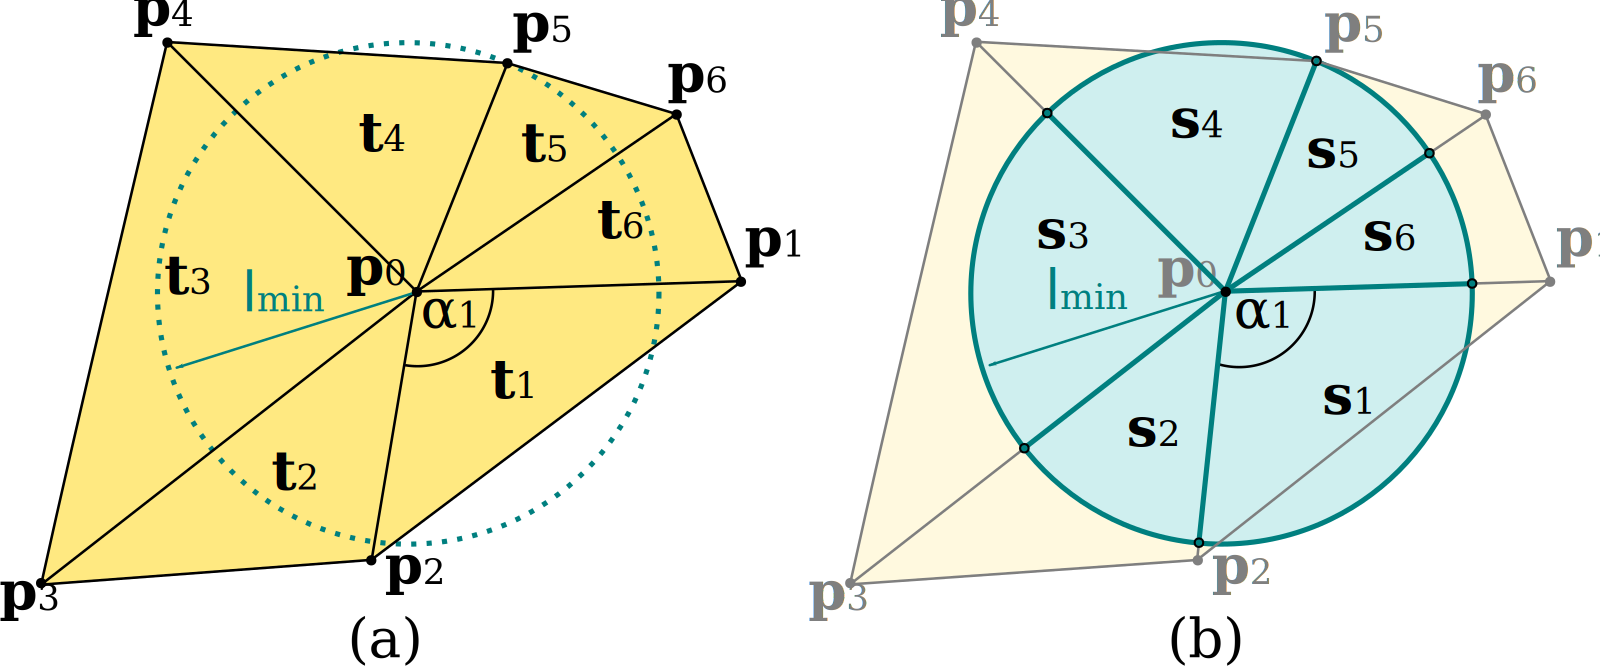
\includegraphics[width=1.0\linewidth]{figures/geodesicDisc.png}}
	{\caption[One-ring and geodesic disc]{A typical configuration of one-ring neighborhood $\bN_v$, described by (a) the six irregular triangular faces $\bt_i$ in sand color, which are defined by the six neighboring points $\bp_i$, which are all adjacent to the center point $\bp_0$; the smallest edge length $\elm = \elm(\bp_5) = |\bp_5 - \bp_0|$ illustrated with a teal arrow as the radius of the geodesic disc $\bO_v$, drawn as a dotted circle, also in teal color; and $\alpha_1$ as the central angle of $\bt_1$ (b) the complete geodesic disc $\bO$ composed of all six of the circular sectors $\bs_i$ which it circumscribes.}\label{fig:geodesicDisc}}
\end{figure}%

Furthermore, to ensure that the filter window size remains static for the duration of each convolution\todoResearch{call to question the importance of global minimum edge length in light of the typo found in source}, we define the global minimum edge length as
%
\begin{equation}
	\gelm := \min\left \{\elm(\bp_0) \;|\; \bp_0 \in \bM\,\right \}
	\label{eq:globalMinimumEdgeLength}
\end{equation}%
\nomenclature[jc]{$\gelm$}{the shortest edge length in $\bM$}%
%
and then use $\gelm$, the shortest edge length between any pair of adjacent points in the triangle mesh $\bM$, in lieu of the local minimum edge length $\elm(\bp_i)$, as the radius of the geodesic disc for all neighborhoods in all the following equations presented in this chapter.

%
%
%
\section{Interior Angles}
\label{ch4sIA}
Having determined the global minimum edge length $\gelm$ in the previous section, we may now consider the next steps in calculating \Fors{t}. Because we intend to use the area of each circle sector $\bs_i$ comprising the geodesic disc $\bO_v$ as weights upon the scalar field $\bF$ for averaging the function values first per sector, and then per neighborhood, we must initially calculate for use in those later computations, the central angles $\alpha_i$ of each triangular face $\bt_i$ in the neighborhood $\bN_v$. These central angles may be obtained by applying the Law of Cosines~\cite{Weisstein19e}, which would yield
%
\begin{equation}
	\alpha_i := cos^{-1}\left (\frac{|\bp_0 - \bp_{i}|^2 + |\bp_0 - \bp_{\sipo}|^2 - |\bp_i - \bp_{\sipo}|^2}{2\cdot|\bp_0 - \bp_{i}|\cdot|\bp_0 - \bp_{\sipo}|}\right )
\end{equation}
%
or more compactly:
%
\begin{equation}
	\alpha := cos^{-1}\left (\frac{\ell_c^2 + \ell_b^2 - \ell_a^2}{2\cdot\ell_c\cdot\ell_b}\right )
	\label{eq:alphaFromEdgeLengths}
\end{equation}%
\nomenclature[ka]{$\alpha$}{the central angle of circle sector $\bs_i$}%

Also, as it is our intention to interpolate and extrapolate the function values in relation to the distances between them and each of their adjacent points in the current neighborhood, we will be required to perform some calculations one side of the sector-bisecting line at a time, as will be discussed in detail later, in Section~\ref{ch4sWM}. But now, having computed the central angles $\alpha$, we can calculate the other interior angles $\beta$, in relation to $\gelm$ and opposite the bisecting line, using the line tangent to the circle sector at the bisecting line, to create two proxy right triangles, which together comprise the larger isosceles triangle which circumscribes the sector $\bs_i$. Next, we can to apply the third angle theorem\footnote{otherwise known as the Angle-Angle-Angle Theorem, abbreviated as AAA}~\cite{Weisstein19f} with $\alpha/2$, to calculate $\beta$ as defined in the formula
%
\begin{equation}
	\beta := \Big(\frac{\pi}{2} - \frac{\alpha}{2}\Big) = \frac{(\pi - \alpha)}{2}
	\label{eq:betaFromHalfAlpha}
\end{equation}%
\nomenclature[kb]{$\beta$}{the third angle with $\frac{\alpha}{2}$ and $\frac{\pi}{2}$}%
\nomenclature[]{$\bp'_j$}{also $\bp'_{\sjpo}$, the corners of the isosceles triangle circumscribing the circle sector, the intermediate location to where $f_j$ is first interpolated or extrapolated}%

Figure~\ref{fig:anglesAndCenterOfGravity} (a) extends Figure~\ref{fig:geodesicDisc} by focusing on the circle sector $\bs_1$, showing the triangular face $\bt_1$, angles $\alpha$ and $\alpha/2$, the bisecting line, the two angles $\beta$ with the tangent line, proxy right triangles defined by the points $\bp'_1$ and $\bp'_2$ used in their calculation, and additionally, the center of gravity which is discussed in detail in the next section.

%
%
%
%
\section{Area \& Center of Gravity}
\label{ch4sIACG}
The next step towards the goal of computing the \wmfv{s} of the circle sectors $\bs_i$, is to calculate for each sector, the area $A$ and the distance $\check{\ell}$ from the center point $\bp_0$ along the bisecting line to the center of gravity $\bc$. Because a circle sector may be defined entirely by its radius and central angle~\cite{Weisstein19d}, having now calculated the radius as $\gelm$ in Section~\ref{ch4sSEL} and the central angle $\alpha$ in Section~\ref{ch4sIA}, the area of a sector can be calculated using the formula
%
\begin{equation}
	A := \frac{\left (\,\gelm\,\right )^2\alpha}{2}
	\label{eq:circularSectorArea}
\end{equation}

Similarly $\check{\ell}$, the distance from the center point $\bp_0$ along the bisecting line to the center of gravity $\bc$, can be calculated directly using the formula
%
\begin{equation}
	\check{\ell} := \frac{4\:\gelm\:\sin(\frac{\alpha}{2})}{3\,\alpha}
	\label{eq:distToCoG}
\end{equation}%

Figure~\ref{fig:anglesAndCenterOfGravity} (a) extends Figure~\ref{fig:geodesicDisc} by enhancing the circle sector $\bs_1$ to illustrate the center of gravity $\bc$ and $\check{\ell}$, the distance along the bisecting line from $\bp_0$ to $\bc$. In general, while holding the radius constant, the closer to $\pi/2$ the central angle $\alpha$ becomes, the longer the distance $\check{\ell}$ will be.

\begin{figure}[ht]
\ffigbox
	{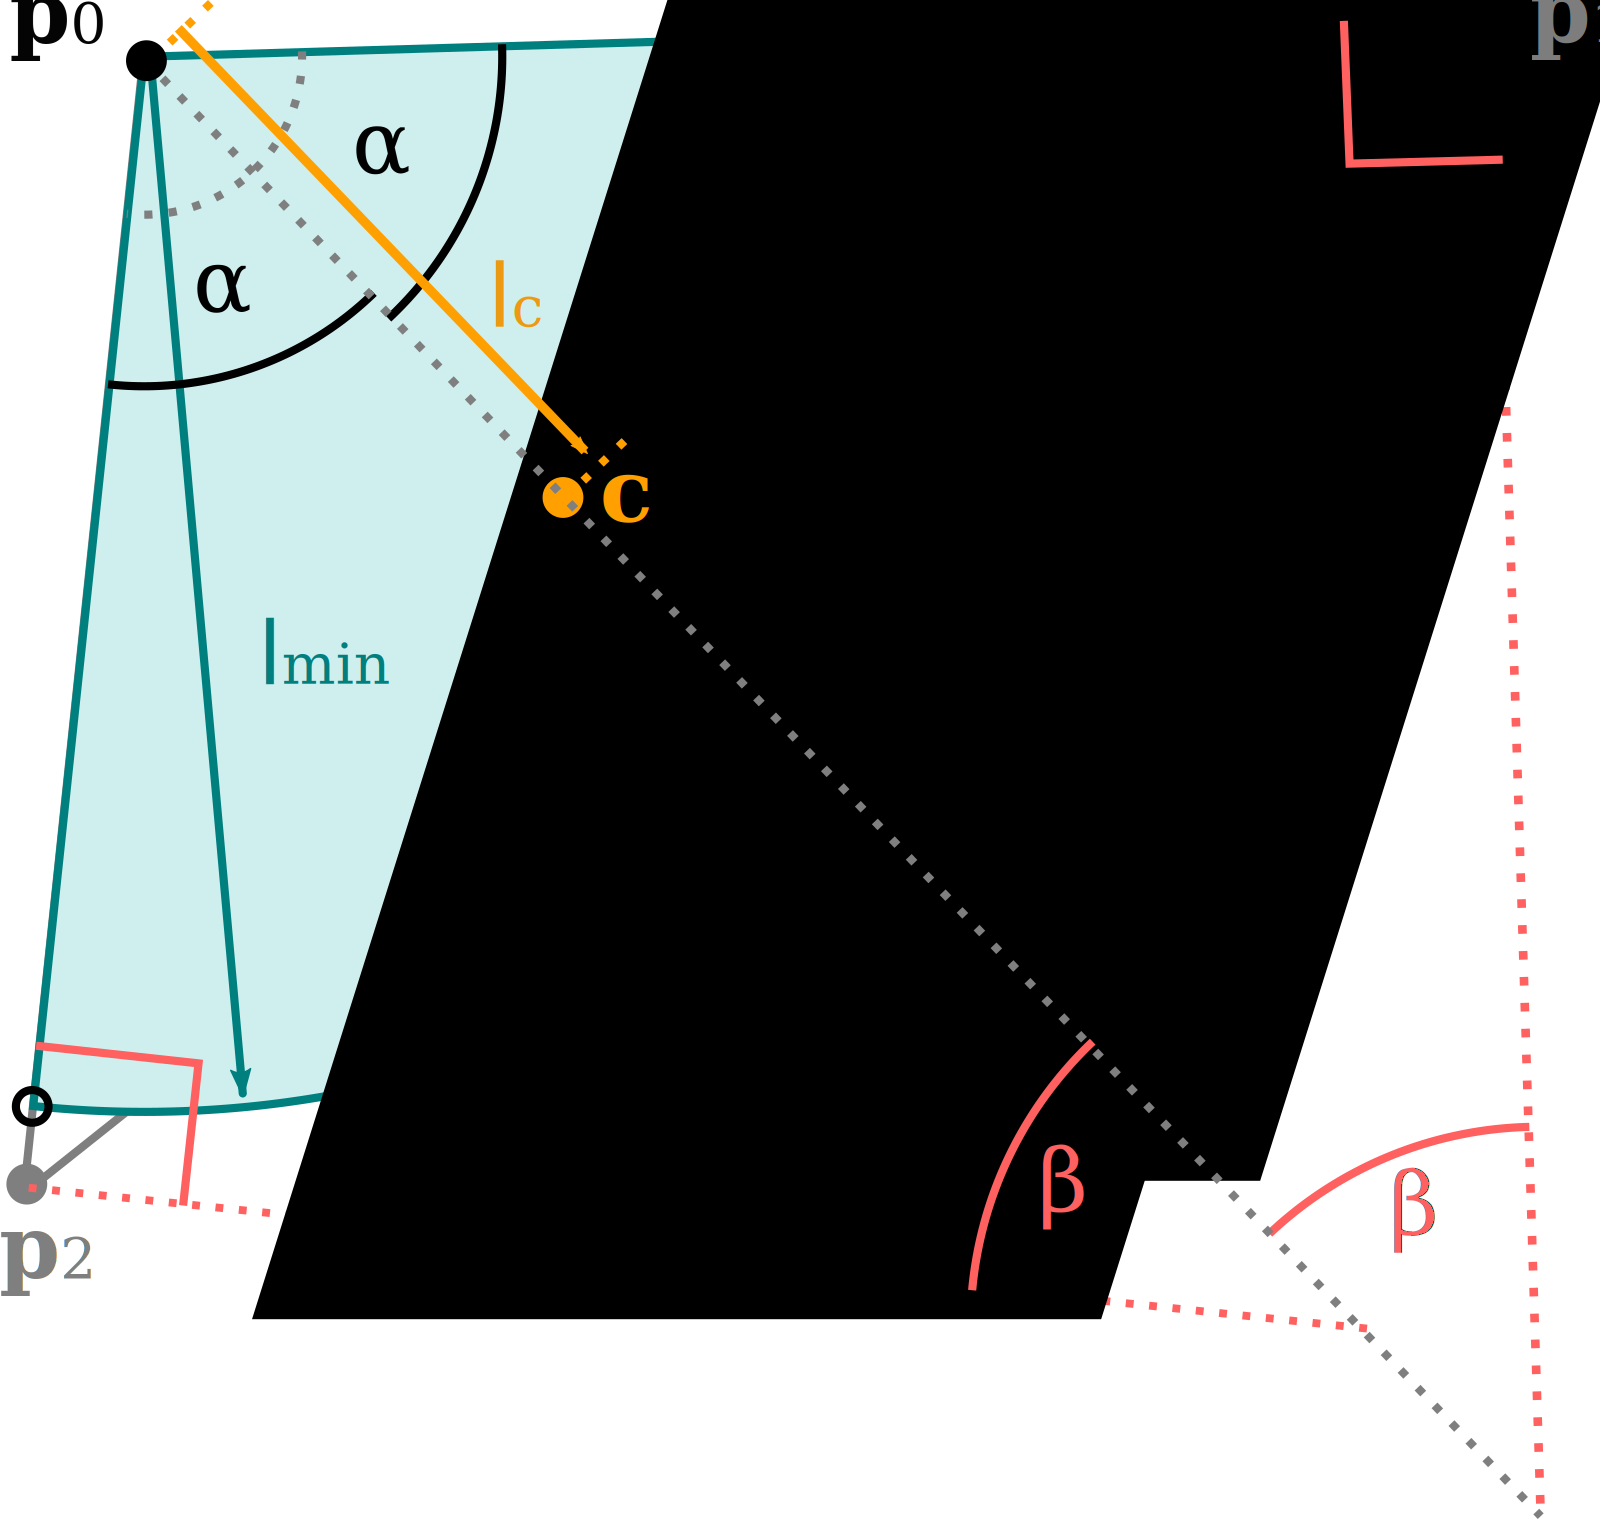
\includegraphics[width=0.8\linewidth]{figures/anglesAndCenterOfGravity.png}}
	{\caption[Angles and Center of Gravity]{An enhanced view of Figure~\ref{fig:geodesicDisc}, focusing on (a) the circle sector $\bs_1$, showing the triangular face $\bt_1$ and points $\bp_1$ and $\bp_2$ in gray, with $\alpha$ and the bisecting line in gray dots. In coral color is the center of gravity $\bc$ and $\check{\ell}$, the distance to it from $\bp_0$ along the bisecting line. Shown in sand color are the angles $\beta$, with the proxy right triangles defined by the points $\bp'_1$ and $\bp'_2$ used in their calculation (b) an example of a face and sector requiring both interpolation and extrapolation of its function values}\label{fig:anglesAndCenterOfGravity}}
\end{figure}%

%
%
%
%
\section{Interpolation \& Extrapolation}
\label{ch4sIE}
With the goal of computing the \wmfv{s} of the circle sectors $\bs_i$ by interpolating and extrapolating the function values from their points towards the center of gravity of each sector $\bc$, in Section~\ref{ch4sSEL} we calculated the global minimum edge length $\gelm$, then in Section~\ref{ch4sIA} we calculated the interior angle $\beta$; both of which are constant between the two halves of the circle sector. So now, given that information, we can obtain the sector-wise constant ratio $\zeta$, which will be used to scale the function values at the points $\bp_i$, to the interpolated or extrapolated values at the corners of the circumscribing isosceles triangle $\bp'_i$, by applying the Law of Sines~\cite{Weisstein19g} and ascribing
%
\begin{equation}
	\zeta := \frac{\gelm}{\sin\left (\beta\right )} = \frac{|\bp'_i - \bp_0|}{\sin\left (\pi/2\right )} = |\bp'_i - \bp_0|
	\label{eq:zeta}
\end{equation}%
\nomenclature[la]{$\zeta$}{sector-wise constant ratio for interpolation derived from Law of Sines}%

For the next few steps in the process of interpolating and extrapolating the function values, we must begin calculating for each half of the circular sector individually, because the points $\bp_j$ and $\bp_{\sjpo}$ are likely\footnote{One need only to look at Figures~\ref{fig:geodesicDisc} or~\ref{fig:anglesAndCenterOfGravity} for an example of why that may be.} at different distances from the center point $\bp_0$. Therefore, while the index $i$ will remain the index of the circle sector $\bs_i$, we will now use the index $j$ to denote the side of the bisecting line, defined by its point $\bp_j$ or $\bp_{\sjpo}$. 

Next, by dividing the sector-wise constant ratio $\zeta$ by the distances to the original points $\ell_j$ and $\ell_{\sjpo}$, we can determine the scalar values with which we can multiply the function values $f_j$ and $f_{\sjpo}$ in order to interpolate or extrapolate them to the corners of the circumscribing isosceles triangle at points $\bp'_j$ and $\bp'_{\sjpo}$. Therefore, these two scalar values are defined as 
\begin{align}
	\tilde{\ell}_j & := \kern2pt\frac{\zeta}{\kern2pt\ell_j\kern2pt}\kern1pt = \kern3pt\frac{\zeta}{|\bp_j - \bp_0|}
	\label{eq:distanceIForInterpolation}\\
	\tilde{\ell}_{\sjpo} & := \frac{\zeta}{\ell_{\sjpo}} = \frac{\zeta}{|\bp_{\sjpo} - \bp_0|}
	\label{eq:distanceIp1ForInterpolation}
\end{align}%
\nomenclature[lb]{$\tilde{\ell}_j$}{also $\tilde{\ell}_{\sjpo}$, the distances for interpolation of $f_j$ and of $f_{\sjpo}$ towards $f_0$}%

Then, by taking the function values\footnote{\fors{T} is agnostic to the meaning of information represented by the data stored as function values in scalar fields, therefore, it can similarly convolve any such data. However, because the filter was designed to only convolve scalar fields, any multi-dimensional data, such as RGB color, must be processed individually as independent scalar fields.} from the scalar field $\bF$, and summing the products of the multiplications between the function values $f_j$, and $f_{\sjpo}$ and their scalar values $\tilde{\ell}_j$ and $\tilde{\ell}_{\sjpo}$, plus the product of the multiplication between the function value at the central point $f_0$ and the complement of each side's scalar value, we can now interpolate and extrapolate the function values at $\bp'_j$ and $\bp'_{\sjpo}$ as


\begin{align}
	f'_j & := f_0\,(1 - \tilde{\ell}_j) + f_j\,\tilde{\ell}_j
	\label{eq:interpolatedFi} \\
	f'_{\sjpo} & := f_0\,(1 - \tilde{\ell}_{\sjpo}) + f_{\sjpo}\tilde{\ell}_{\sjpo}
	\label{eq:interpolatedFip1}
\end{align}%
\nomenclature[lc]{$f'_j$}{also $f'_{\sjpo}$, the interpolated values of $f_j$ and $f_{\sjpo}$ toward $f_0$}%
\todoStyle{should I be using the $\bff$ macro?}

Figure~\ref{fig:interpolatedFunctionValues} illustrates a 3D-projected, enhanced view of the circle sector $\bs_1$, continuing with the example introduced in Figure~\ref{fig:geodesicDisc}. Drawn above the points $bp_0$, $bp_1$, and $bp_2$ are the three function values $f_0$, $f_1$, and $f_2$ from the scalar field $\bF$, with the heights indicative of each function value's magnitude. Also shown are the extrapolated function values $f'_0$, and $f'_1$ above the corners of the isosceles triangle $\bp`_1$, and $\bp`_1$, as well as the dotted lines illustrating the vectors on which the extrapolated values were calculated. Furthermore, it illustrates the process of interpolating of the extrapolated function values towards each other, and then again towards the center of gravity, which is the topic of the next section.

\begin{figure}[ht]
\ffigbox
	{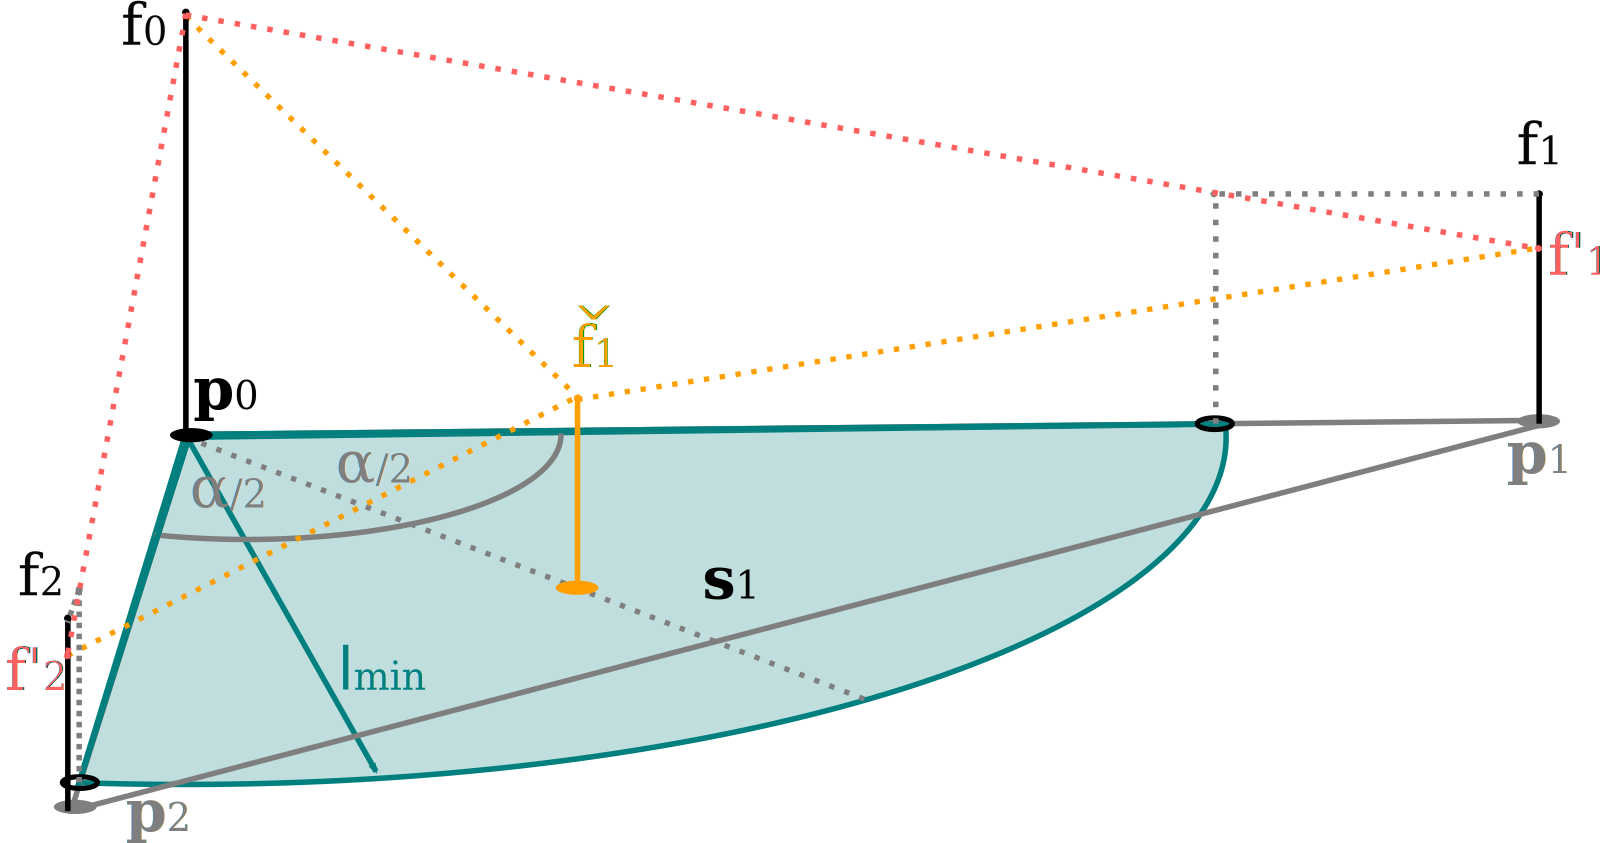
\includegraphics[width=1.0\linewidth]{figures/interpolatedFunctionValues}}
	{\caption[Interpolation of Function Values toward the Center of Gravity]{An enhanced view...}\label{fig:interpolatedFunctionValues}}
\end{figure}

%
%
%
%
\section{Weighted Means}
\label{ch4sWM}
Now that we have, in Section~\ref{ch4sACG}, calculated the distance to the center of gravity of each circle sector $\check{\ell}$, and then in Section~\ref{ch4sIE}, computed the two function values interpolated or extrapolated to the corners of the isosceles triangle circumscribing the circle sector, $f'_j$ and $f'_{\sjpo}$, we are now poised to begin the computation of the \wmfv{s}, first for each circle sector $\bs_i$, then for the entire geodesic disc $\bO_v$, and finally iteratively convolving \Fors{t} over the entire mesh to generate the smoothed, scalar field of \wmfv{s} $\bF'$.

In order to calculate the weighted mean function value at the center of gravity $\bc$, of the circle sector $\bs_i$, we must combine the original function value at the center point $f_0$, and both interpolated function values, $f'_j$ and $f'_{\sjpo}$. Then using the distance to the center of gravity $\check{\ell}$, and the formula
\begin{equation}
	\check{f} = f_0\,(1 - \check{\ell}) + \frac{(f'_j + f'_{\sjpo})\,\check{\ell}}{2}
	\label{eq:weightedMeanAtCoGatSector}
\end{equation}%
\nomenclature[ma]{$\check{f}$}{the weighted mean function value at $\bc$ of $\bs_i$}%
we obtain the weighted mean function value $\check{f}$, at the center of gravity, representing the entire circle sector.

Figure~\ref{fig:interpolatedFunctionValues} illustrates $\check{f}_1$ in sand color as a volume over an enhanced view of the circle sector $\bs_1$, continuing with the example introduced in Figure~\ref{fig:geodesicDisc}. The figure also shows details pertaining to the interpolation of the function values $f_j$ and $f_{\sjpo}$, as discussed in detail in Section~\ref{ch4sI}.
\todoReword{update after changes to figure}


Finally, we can multiply each interpolated function value located at each circle sector's center of gravity $\check{f}_i$, by each sector's area $A_i$, to obtain a volume of function value over the entire circle sector. Then by dividing the sum of all those sector-wise function value volumes by the total area of the geodesic disc $\bO_v$, we can compute
\begin{equation}
	f'_v := \frac{\sum A_i\check{f}_i}{\sum A_i} \quad \forall i \in \{1,\ldots,\,|\bN_v|\}
	\label{eq:meanFuncValAtPv}
\end{equation}%
\nomenclature[mb]{$f'_v$}{the one-ring weighted mean function value at $\bp_v$}%
the one-ring weighted mean\footnote{\fors{T} can be modified to use the median operation, instead of the mean, by using all the equations except Equation~\ref{eq:meanFuncValAtP0} and then sorting the results of Equation~\ref{eq:weightedMeanAtCoGatSector}. The details of which can be found by the original publication ~\cite[s.~3.2]{Mara17}, but as it was not implemented in GPGPU for this thesis, we exclude the details here.} function value for $\bp_v$, which is the center point $\bp_0$ of the neighborhood $\bN_v$.

Figure~\ref{fig:funcValVolumes} illustrates the geodesic disc $\bO$, as introduced in Figure~\ref{fig:geodesicDisc}, with volumes of interpolated function value over each circle sector, which shall be divided by each sector's area in order to obtain the the one-ring weighted mean function value $f'_v$ at $\bp_v$.
\begin{figure}[ht]
\ffigbox
	{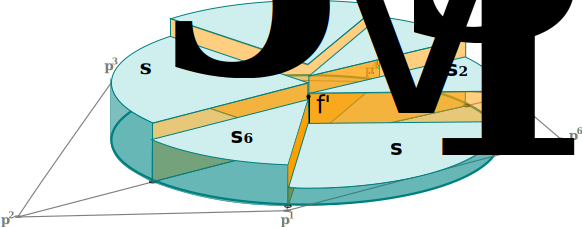
\includegraphics[width=1.0\linewidth]{figures/funcValVolumes.png}}
	{\caption[Weighted Mean Function Value $f'_v$at $\bp_v$]{The geodesic disc $\bO$, as introduced in Figure~\ref{fig:geodesicDisc}, with volumes of interpolated function values over each circle sector $\bs_i$, which shall be divided by each sector's area $A$ in order to obtain the the one-ring weighted mean function value $f'_v$ at $\bp_v$.}\label{fig:funcValVolumes}}
\end{figure}

As with any smoothing filter, there is no upper limit to the count of iterations one can convolve, however, the function values will all eventually converge at the global mean average function value. More details can be found in Section~\ref{ch3s2}.\todoCitation{mara on iteration count vs filter size}.\todoReword{elaborate}

%
%
%
\section{Summary}
\label{ch4sS}
In this chapter we presented an updated version of \Fors{t}, which since its original publication~\cite[s.~3.2]{Mara17}, now utilizes the entire area of each sector $\bs$ of the geodesic disc $\bO$ centered at each point $\bp_v$ in the mesh $\bM$, in order to calculate the weighted average of all the function values in its one-ring neighborhood. First, we illustrated in detail how one can calculate the globally shortest edge length $\gelm$, interior angles $\alpha$ and $\beta$, the area $A$, and the distance $\check{\ell}$ from the center point to the center of gravity $\bc$, for any given of circle sector in a one-ring neighborhood $\bN$. Next, we provided the equations for interpolating the three function values $f_0$, $f_j$, and $f_{\sjpo}$, using the pairwise constant ratio $\zeta$ in order to obtain the weighted mean function value $\tilde{f}$ for each $\bs$, and finally the weighted mean function value $f'_v$ at point $\bp_v$, representing the entire one-ring neighborhood $\bN$. Convolving this filter at each vertex in the mesh, with the scalar field of function values $\bF$, for any number of iterations, thus produces a smoothing effect with increasing intensity in relation to the number of iterations.
